\documentclass{article}
\usepackage{graphicx}
\usepackage{float}

\title{CMSC6950 Project Report: Tidynamics}
\author{Karina Barcelos}
\date{Spring - June 2021}

\setlength{\oddsidemargin}{0.5cm}
\setlength{\textwidth}{15.5cm}
\setlength{\topmargin}{-1.5cm}
\setlength{\textheight}{22cm}

\begin{document}
\maketitle

\section{Introduction}

Tidynamics \cite{Buyl2018} is a tiny and simple package that calculates mean-square displacements (MSD) of a trajectory and correlation functions of a input data using the Fast Correlation Algorithm, being \cite{kneller1995nmoldyn} especially beneficial for quantitatively evaluating dynamics of stochastic and molecular simulations from time-dependent numerical trajectories. The MSD is a deviation of the position of a certain particle regarding a reference position at time intervals. Whereas the other useful computational tools of this software are the autocorrelation function (ACF) and correlation function, in which both are conceptually similar, i.e, mathematical representations of similarity degree. ACF uses a variable with itself between two successive at two points in time (time lags) and correlation function is the relationship between two different time series at successive time lags.
 
The data format input and output of tidynamics \cite{Buyl2018} is array, simply depending only on Python and NumPy. The NumPy arrays where the first index indicates the timestep and the second index, in case of correlation function between two time-series, shows the spatial coordinates of the trajectory. Both ACF and MSD are defined by the respective Equations 1 and 2 below in tidynamics algorithm \cite{Buyl2018}, where the angle brackets denote an average over time. \cite{kneller1995nmoldyn}

\begin{equation}
C_{AB}(\tau) = \langle A(0) B(\tau) \rangle,
\label{eqn:correlation}
\end{equation}
where  $A(0)$ and $B(\tau)$ represent the input data quantity A and the quantity at some later time B, respectively. $C_{AB}$ saved the ACF value.

\begin{equation}
MSD(\tau) = \langle (x(\tau) - x(0) )^2 \rangle,
\label{eqn:msd}
\end{equation}
where $x(\tau)$ and $x(0)$ refer to current and reference positions, respectively.

The aim of this project was to implement two computational tasks of dynamical systems from the chosen open source package tidynamics \cite{Buyl2018}. For the first task, the ACF was computed for the bond length of C-H and C=O from a certain Tyrosine over 700 ns of my input Molecular Dynamics (MD) simulation data of a certain protein. It has been chosen to work with a more applicable input data to test that function in a real MD system. For the second task, the random walk values from coordinates x = cos $\theta$ and y sin = $\theta$ with angle $\theta$ between 0 $\leq$ $\theta$ $\leq$ $2\pi$ in a range of N = 1000 steps and its 2D random walk MSD were generated. Several modules were utilized during the project, including numpy, pandas, math, sys, and matplotlib.

\section{Results}

The results will be reported for use of ACF and MSD from tidynamics package \cite{Buyl2018}.

\subsection{Task 1: ACF of C=O and C-H bond length over MD time}

The objective of this task was to analyze the C=O and C-H bond stretching motion using its time ACF. The input data were obtained from a long MD simulation trajectory with total duration of 1.5 ms of a Tyrosine amino acid of a certain protein. A MD simulation is a computer simulation method that allows to predict and visualize at atomistic level the motion of a system (often a protein) of time evolution. The time evolution herein was in nanosecond (ns) from a period of 800-1500 ns to ensure data analysis in the protein equilibrium; however, the plot was limited to 800-1000 ns to better visualization. The final input files had the C=O and C-H bond lengths in nanometer (nm) over 200 ns time series and an autocorrelation function calculated from tidynamics \cite{Buyl2018}in a time-series. In the ACF first script, it loaded the data, time and length and those values were converted into a dataframe. The result dataframe after applying the ACF in C-H and C=O lengths were added to a new column in the dataframe. The ACF first sript resulted in two txt intermediate files, each one for each type of bond (i.e., CH and CO). The ACF second script utilized these output files for loading and plotting the Figure ~\ref{fig:acf_plot}. The ACF showed near zero positive autocorrelation for those bond length data, which do not vary drastically over a long period of simulation.

\begin{figure}[H]
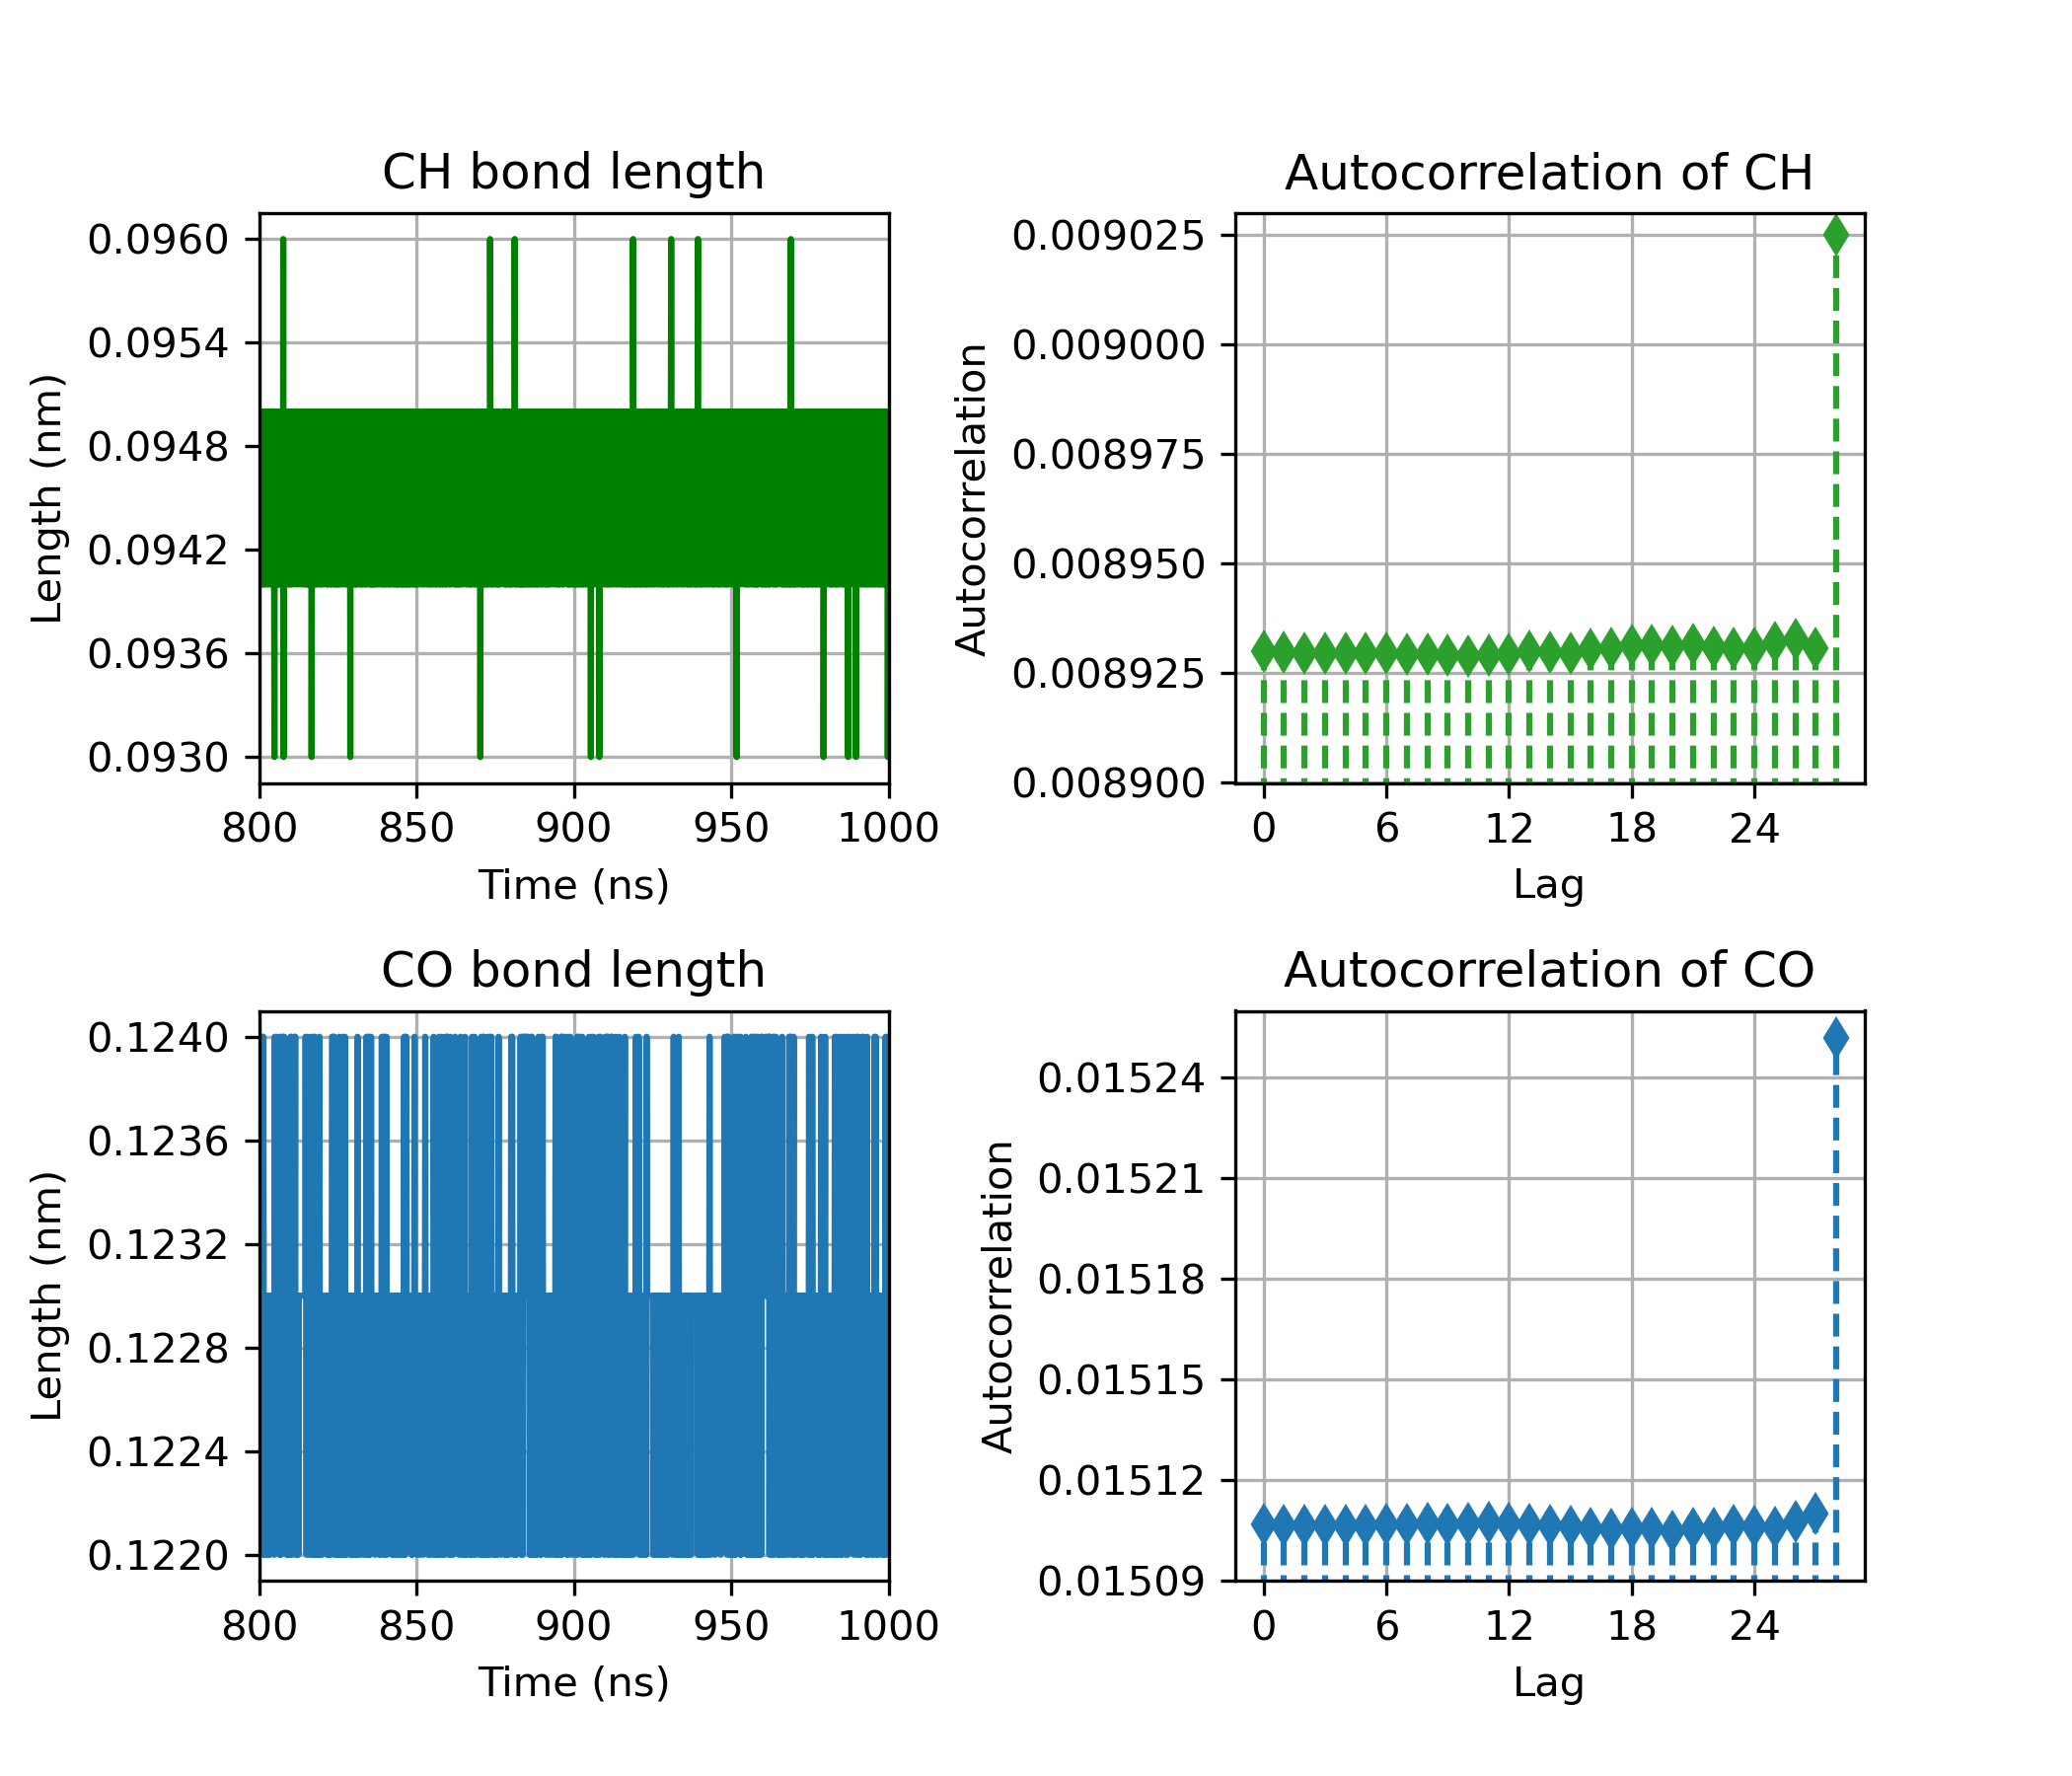
\includegraphics[width=\linewidth]{CO_CH_length_acf_plot.png}
\caption{C-H and C=O bond length from a Tyrosine amino acid over MD simulation time and their ACF after 800 ns to ensure the system is in equilibrium.}
\label{fig:acf_plot}
\end{figure}

\subsection{Task 2: MSD of a random walk}

For the second computational task, it was generated a random walk of 1000 steps. In the first MSD script, by starting with an example with a certain walker at the origin, (x,y), it then chooses a random direction between 0 $\leq$ $\theta$ $\leq$ $2\pi$ for the first step of the walk. For that, it is necessary to determine a random angle value number using a random-number generator in order to the sequence of random numbers do not probably repeat in each further random walk step. In case of this task script, a random value was obtained after a random angle was applied in x and y coordinates, such as x = cos $\theta$ and y = sin $\theta$. For each of N step, those prior values were calculated to the cumulative values for x and y being updated for each step. Then the (x,y) values were saved into an array and after a dataframe. The MSD were applied in x and y as it is a 2D position dataset. The Figure ~\ref{fig:msd_plot} was then plotted from the second MSD script, containing the 2D random walk coordinates with start and end markers and its numerical and theoretical MSD curves. The theoretical MSD value for a random walk is linear to time (in this casem, N=1000), according to Equation \ref{eqn:msd2}. If we start with lots of coordinates at a certain origin at time zero, the mean position of the coordinates does not change with time but the distribution of coordinate positions around the origin spreads with time. Thus, time is multiplied by 2 to obtain the theoretical MSD.

\begin{equation}
MSD(\tau) \approx 2 D \tau
\label{eqn:msd2}
\end{equation}
where D and t are difusion constant and time, respectively.


\begin{figure}[H]
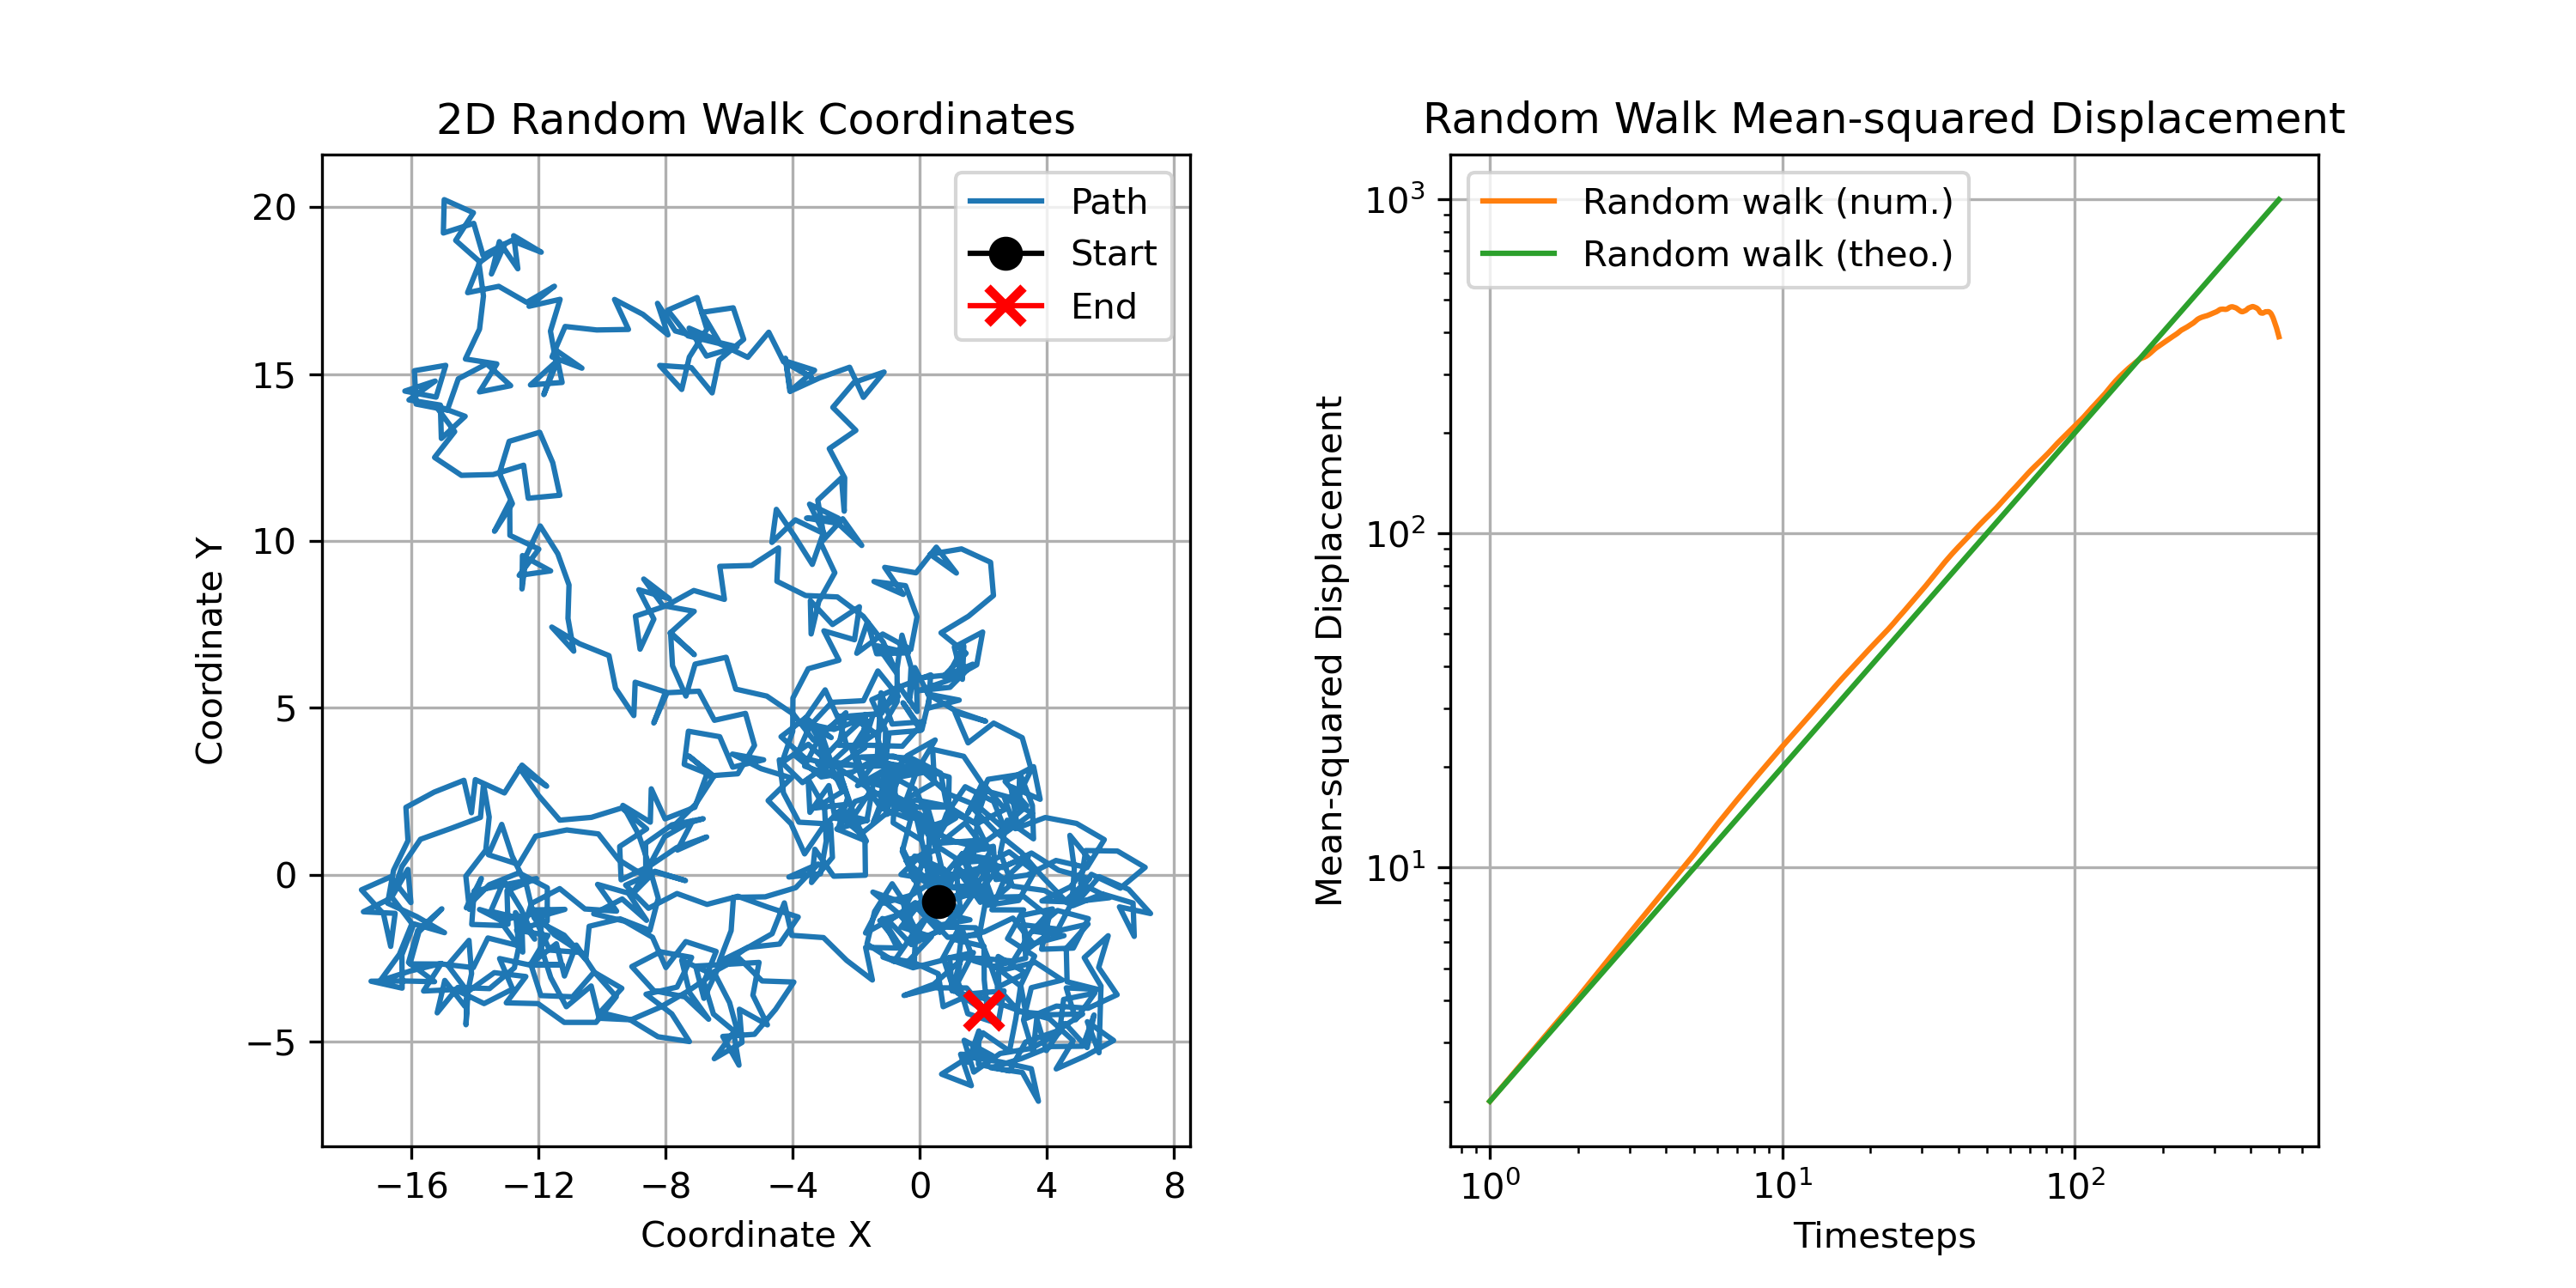
\includegraphics[width=\linewidth]{msd_plot.png}
\caption{2D random walk in a (x,y) coordinates and its mean-squared displacement.}
\label{fig:msd_plot}
\end{figure}

\section{Conclusions}

Therefore, two computational tasks were performed using tidynamics package to calculate its common tools, such as ACF and MSD, and plot their results in different visualizations. The first script of each ACF and MSD were the computational task and the seacond of each were their visualization plotting-related script. The first task provided a figure of the bond length of C-H and C=O and its ACF over 700 ns a MD dynamics simulation, data obtained from a trajectory of a Tyrosine. It required tidynamics, numpy, matplotlib, and pandas python libraries. Whereas the second task, MSD of a random walk was plotted, in which x and y coordinates were applied cosine (theta) and sine (theta) while theta was randomly sorted in the direction between 0 $\leq$ $\theta$ $\leq$ $2\pi$. For that, it was used numpy, math, tidynamics, matplotlib, and pandas libraries.

\bibliographystyle{plain}
\bibliography{references}

\end{document}
